\documentclass[10pt,a4paper]{article}
\usepackage[margin=2cm]{geometry}
\usepackage[T1]{fontenc}
\usepackage[utf8]{inputenc}
\usepackage{lmodern}
\usepackage{graphicx}
\usepackage{booktabs}
\usepackage{caption}
\usepackage{hyperref}
\usepackage{xcolor}
\newcommand{\BestBlockSize}{128}
\newcommand{\CpuFitExponent}{1.91}
\newcommand{\GpuFitExponent}{0.85}
\newcommand{\MaxRelDrift}{$1.73\times 10^{-4}$}
\newcommand{\CpuDoublingMin}{3.61}
\newcommand{\CpuDoublingMax}{3.88}
\newcommand{\GpuDoublingMin}{1.71}
\newcommand{\GpuDoublingMax}{1.89}
\newcommand{\SpeedupDoublingMin}{2.05}
\newcommand{\SpeedupDoublingMax}{2.11}


\title{Lennard--Jones CUDA benchmark report}
\author{Nejc Krajšek, Rok Mušič}
\date{May 2026}

\begin{document}
\maketitle
\vspace{-1.5em}

We benchmarked the final code on 5000 simulation steps for $N=1000, 2000, 4000$ and $8000$ particles. The block-size sweep used GPU block sizes 64, 128, 256, 512 and 1024. For the final CPU vs GPU comparison we used block size \BestBlockSize, because it was the fastest choice in every tested case. We implemented all the requirements for the basic grades, but none of the optional ones for a higher grade.

\paragraph{Block-size sweep.}
Table~\ref{tab:block} shows the mean GPU time for each tested block size. We found out that block size \BestBlockSize is the best choice for all four particle counts. Block size 64 is very close, which means that the kernel already has enough parallel work in that range. From block size 256 onward the runtime gets worse, and at 1024 it gets much worse. We interpret this as a simple balance issue: very large blocks give each launch less flexibility, so the GPU has a harder time keeping enough useful work active at the same time. For 8000 particles, we ran only one measurement for each block size, and 128 was still the fastest choice.

\begin{table}[h]
    \centering
    \caption{Mean GPU runtime [s] for the block-size sweep at 5000 steps. Best time in each row is bold.}
    \label{tab:block}
    \small
    \begin{tabular}{rccccc}\toprule
$N$ & 64 & 128 & 256 & 512 & 1024 \\ \midrule
1000 & 2.783 & \textbf{2.738} & 2.864 & 3.676 & 6.590 \\ 
2000 & 4.707 & \textbf{4.688} & 4.813 & 5.840 & 10.551 \\ 
4000 & 8.545 & \textbf{8.459} & 8.720 & 10.298 & 18.244 \\ 
8000 & 16.026 & \textbf{15.972} & 16.614 & 19.335 & 33.439 \\ 
\bottomrule\end{tabular}

\end{table}

\paragraph{Final timing results and speed-up.}
Table~\ref{tab:basic} gives the final CPU and GPU timings and the resulting speed-up. We found out that the GPU is already faster at $N=1000$ by $11.49\times$, and that the advantage grows strongly with problem size, reaching $103.80\times$ at $N=8000$. This trend is stable across the whole range: every time we doubled $N$, the CPU time increased by about \CpuDoublingMin{}--\CpuDoublingMax$\times$, while the GPU time increased by only about \GpuDoublingMin{}--\GpuDoublingMax$\times$. As a result, the speed-up itself increased by about \SpeedupDoublingMin{}--\SpeedupDoublingMax$\times$ for each doubling of $N$.

\begin{table}[h]
    \centering
    \caption{Final benchmark results at 5000 steps using GPU block size \BestBlockSize.}
    \label{tab:basic}
    \small
    \begin{tabular}{rccc}\toprule
$N$ & CPU time [s] & GPU time [s] & Speed-up \\ \midrule
1000 & 31.460 $\pm$ 0.025 & 2.739 $\pm$ 0.002 & $11.49\times$ \\ 
2000 & 113.443 $\pm$ 0.016 & 4.691 $\pm$ 0.002 & $24.18\times$ \\ 
4000 & 427.440 $\pm$ 0.047 & 8.457 $\pm$ 0.002 & $50.54\times$ \\ 
8000 & 1658.600 $\pm$ 0.000 & 15.979 $\pm$ 0.003 & $103.80\times$ \\ 
\bottomrule\end{tabular}

\end{table}

Figure~\ref{fig:scaling} shows the same data on a log--log scale together with simple power-law fits. We found out that the CPU measurements follow an empirical trend close to $N^{\CpuFitExponent}$, which matches the expected strong growth of the all-pairs force computation ($O(n^2)$ in theory). The GPU fit is much flatter, about $N^{\GpuFitExponent}$ over the measured range. We do not claim that the true complexity changed; instead, this shows that the GPU overhead is better hidden as the problem gets larger (a similar trend to what we observed in the previous homework (a similar trend to what we observed in the previous homework). The speed-up plot on the right confirms the same story in a direct way: larger systems use the GPU more effectively.

\begin{figure}[h]
    \centering
    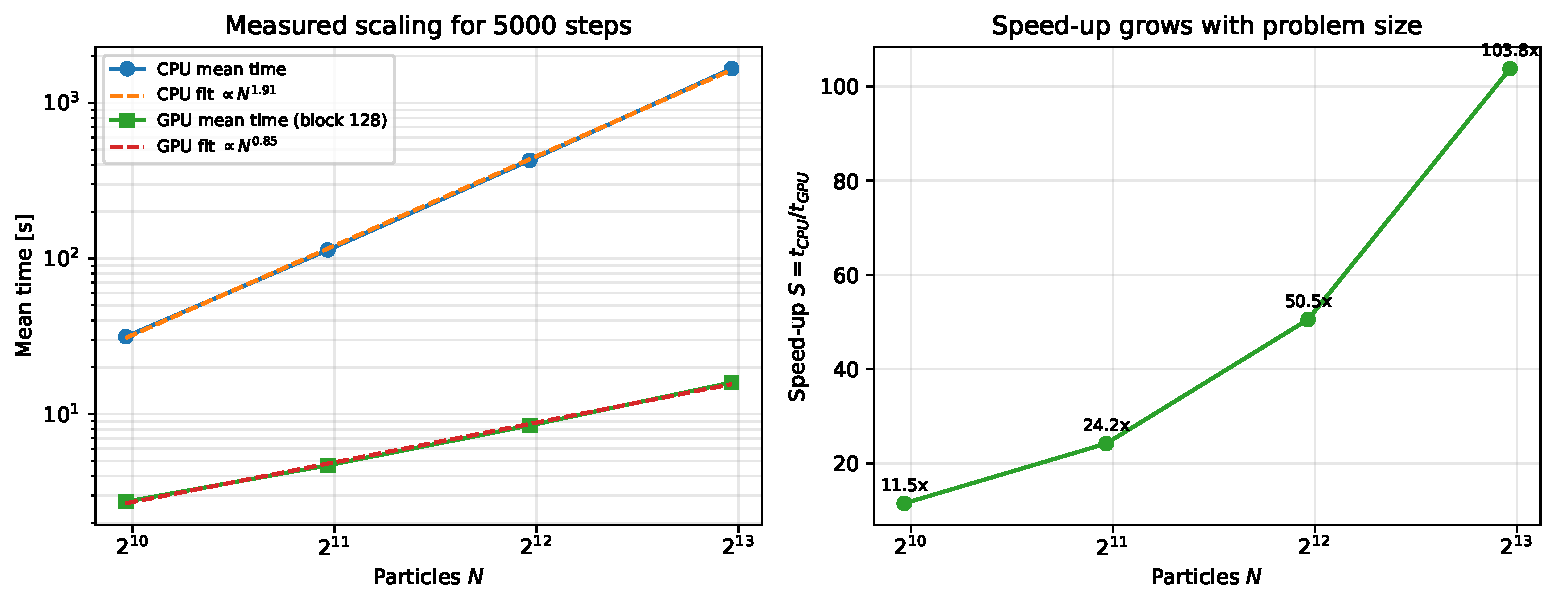
\includegraphics[width=0.98\linewidth]{figures/scaling_and_speedup.pdf}
    \caption{Left: measured CPU and GPU scaling with simple empirical power-law fits. Right: speed-up increases steadily with particle count.}
    \label{fig:scaling}
\end{figure}

\paragraph{Correctness check.}
We also checked energy conservation. The mean relative total-energy drift stayed below \MaxRelDrift{} for every reported CPU and GPU case. The absolute drift grows with $N$, but the relative drift stays small and the CPU and GPU values stay close to each other. We therefore found no sign that the CUDA version changes the physical behaviour in a meaningful way over the measured 5000-step runs. As required, we also stored a separate final state visualization outside the report.

\paragraph{Conclusion.}
We found out that the most important practical choice was the GPU block size, and that 128 threads per block was the best setting in all tested cases. With that choice, the GPU gave a clear speed-up already at 1000 particles and the benefit grew quickly with larger systems. The measured data therefore supports the main conclusion of our work: for this implementation, the GPU version is not only correct, but also much more effective than the CPU baseline once the particle count becomes moderately large.

\end{document}
